%%%%%%%%%%%%%%%%%%%%%%%%%%%%%%%%%%%%%%%%%%%%%%%%%%%%%%%%%%%%%%%%%%%%%%%%%%%%
%               PRIERE DE NE RIEN MODIFIER CI-DESSOUS                      %
%       JUSQU'A LA LIGNE "PRIERE DE NE RIEN MODIFIER CI-DESSUS"            %
%   TOUT LE BLOC QUI SUIT SERA SUPPRIME LORS DE L'EDITION FINALE DU POLY   %
%   CONTENANT LES RESUMES                                                  %
%%%%%%%%%%%%%%%%%%%%%%%%%%%%%%%%%%%%%%%%%%%%%%%%%%%%%%%%%%%%%%%%%%%%%%%%%%%%
\documentclass[10pt]{article}
%===  Priere de ne pas utiliser d'autres modules
\usepackage{latexsym}
\usepackage{bbm}              % fontes doubles (pour les ensembles, par ex.)
\usepackage{graphicx}         % pour d'eventuelles figures
\usepackage{epsfig}           % (preferer graphicx, si possible)
\usepackage{amsmath}          % AMSTEX
\usepackage{amsfonts}
%
\setlength{\paperheight}{297mm}\setlength{\paperwidth}{210mm}
\setlength{\oddsidemargin}{10mm}\setlength{\evensidemargin}{10mm}
\setlength{\topmargin}{0mm}\setlength{\headheight}{10mm}\setlength{\headsep}{8mm}
\setlength{\textheight}{240mm}\setlength{\textwidth}{160mm}
\setlength{\marginparsep}{0mm}\setlength{\marginparwidth}{0mm}
\setlength{\footskip}{10mm}
\voffset -13mm\hoffset -10mm\parindent=0cm
\def\titre#1{\begin{center}{\Large{\bf #1}}\end{center}}
\def\orateur#1#2{\begin{center}{\underline{\large{\bf #1}}}, {#2}\end{center}}
\def\auteur#1#2{\begin{center}{\large{\bf #1}}, {#2}\end{center}}
\def\auteurenbasdepage#1#2#3{\small{\bf #1}, \small{#2}\\ \small{\tt #3}\\ }
\def\motscles#1{%
	\ifx#1\IsUndefined\relax\else\noindent{\normalsize{\bf Mots-cl\'es :}} #1\\ \fi}
\renewcommand{\refname}{\normalsize R\'ef\'erences}
%
\begin{document}
\thispagestyle{empty}
%%%%%%%%%%%%%%%%%%%%%%%%%%%%%%%%%%%%%%%%%%%%%%%%%%%%%%%%%%%%%%%%%%%%%%%%%%%%
%               PRIERE DE NE RIEN MODIFIER CI-DESSUS                       %
%%%%%%%%%%%%%%%%%%%%%%%%%%%%%%%%%%%%%%%%%%%%%%%%%%%%%%%%%%%%%%%%%%%%%%%%%%%%
%
% DANS TOUTE LA SUITE NOUS PRIONS LES AUTEURS DE BIEN VOULOIR UTILISER
% LA SYNTAXE TeX STRICTE POUR LES LETTRES ACCENTUEES.
% ON PEUT AU BESOIN LES REMPLACER APR\'ES LA FRAPPE DU DOCUMENT
% PAR LEUR \'EQUIVALENT TeX.
% DANS LE CAS CONTRAIRE LES LETTRES ACCENTU\'ES N'APPARA\^ITRONT PAS
% DANS LE DOCUMENT FINAL.
%
%                   ORATEUR ET CO-AUTEURS
%---------------------------------------------------------------
%
% LES AUTEURS SONT PRIES DE FOURNIR LES BONS ARGUMENTS AUX MACROS CI-DESSOUS :
%   \Titre         : Titre de la communication
%   \NomOrateur    : Pr\'enom(s) NOM de l'Orateur
%   \AdresseCourteOrateur : Exemple : Universit\'e de Rennes 1
%   \AdresseLongueOrateur : Exemple : IRMAR, Universit\'e de Rennes 1, 263 avenue du G\'en\'eral Leclerc, 35000 Rennes
%   \EmailOrateur : Adresse electronique
%
% ET DE MEME POUR LES EVENTUELS CO-AUTEURS :
%   \NomAuteurI ...
%   \AdresseCourteAuteurI ...
%---------------------------------------------------------------
% DEFINIR ICI LE TITRE DE VOTRE COMMUNICATION
\def\Titre{Couplage de m\'ethodes d'optimisation topologique de formes et d'optimisation de trajectoires en fabrication additive}
%
% DEFINIR ICI LES NOMS, ADRESSES, ... DE l'ORATEUR OU UNIQUE AUTEUR
\def\NomOrateur{Mathilde BOISSIER}
\def\AdresseCourteOrateur{CMAP, LURPA}
\def\AdresseLongueOrateur{CMAP, Ecole Polytechnique, Route de Saclay, 91128 Palaiseau Cedex\\
LURPA, ENS Cachan, 61 avenue du Pr\'esident Wilson, 94 230 Cachan	}
\def\EmailOrateur{mathilde.boissier@cmap.polytechnique.fr}
%
% DEFINIR ICI LES NOMS, ADRESSES, ... DES EVENTUELS CO-AUTEURS
\def\NomAuteurI{Gr\'egoire ALLAIRE}
\def\AdresseCourteAuteurI{CMAP}
\def\AdresseLongueAuteurI{CMAP, Ecole Polytechnique, Route de Saclay, 91128 Palaiseau Cedex }
\def\EmailAuteurI{allaire@cmap.polytechnique.fr}

\def\NomAuteurII{Christophe TOURNIER}
\def\AdresseCourteAuteurII{LURPA}
\def\AdresseLongueAuteurII{LURPA, ENS Cachan, 61 avenue du Pr\'esident Wilson, 94 230 Cachan}
\def\EmailAuteurII{christophe.tournier@lurpa.ens-cachan.fr}

%=== et ainsi de suite II, III, IV, V ... pour les suivants
%
%=== Liste des mots-cles separes par des virgules si besoin
% N'enlever le signe % que si necessaire
%\def\listmotcles{mot-cle-1, mot-cle-2, ...}
%
%
%                   DEBUT DE LA COMMUNICATION
%---------------------------------------------------------------
% NE PAS MODIFIER LA LIGNE SUIVANTE
% Le titre est a definir dans la macro \Titre (23 lignes plus haut)
\titre{\Titre}%
%---------------------------------------------------------------
% TITRE & AUTEUR(S)
% RETIRER LES SIGNES % SI NECESSAIRE ET PLACER DANS L'ORDRE SOUHAITE
% DANS LES LIGNES SUIVANTES NE MODIFIER QUE LES SIGNES COMMENTAIRES '%'
% Les noms, adresses, email de l'orateur et des co-auteurs sont a definir
% dans les macros \NomOrateur, \AdresseCourteOrateur etc. plus haut
%---------------------------------------------------------------
\orateur{\NomOrateur}{\AdresseCourteOrateur}
% NE PAS MODIFIER LES 4 LIGNES SUIVANTES sauf a retirer le signe commentaire '%'
\auteur{\NomAuteurI}{\AdresseCourteAuteurI}
\auteur{\NomAuteurII}{\AdresseCourteAuteurII}

%
\motscles{\listmotcles}
%---------------------------------------------------------------
% TEXTE DE LA COMMUNICATION
%---------------------------------------------------------------


Le proc\'ed\'e de fabrication m\'etallique sur lit de poudre est un proc\'ed\'e de fabrication couche par couche consistant \`a faire fusionner de la poudre au passage d'un laser \cite{ref2}. Ce proc\'ed\'e induit des temp\'eratures qui peuvent \^etre tr\`es \'elev\'ees et varier fortement sur des domaines r\'eduits. Ces ph\'enom\`enes thermiques sont \`a l'origine de d\'eformations m\'ecaniques telles que la distortion et la formation de contraintes r\'esiduelles, entrainant des fragilit\'es dans la pi\`ece construite.  

\vspace{1cm}

Les trajectoires de lasage jouent donc un r\^ole pr\'epond\'erant dans ce type de fabrication additive, car, bien choisies, elles peuvent permettre de minimiser les d\'efauts m\'ecaniques de la pi\`ece. Cependant, pour des raisons de production industrielle, elles doivent aussi satisfaire des contraintes g\'eom\'etriques garantissant un passage rapide du laser lors de la fabrication de la couche.

\vspace{1cm}

L'objectif est  donc de coupler les m\'ethodes d'optimisation g\'eom\'etriques et topologiques de forme (en utilisant la m\'ethode level-set \cite{ref1}) avec des strat\'egies de commande de trajectoires afin, d'une part, en mod\'elisant ces contraintes de lasage, de designer des pi\`eces faciles \`a fabriquer, et d'autre part, d'optimiser la trajectoire de lasage elle-m\^eme, pour permettre d'am\'eliorer la qualit\'e ainsi que la vitesse de fabrication des pi\`eces.

\begin{figure}[h]
	\begin{minipage}{0.45\textwidth}
		\centering
		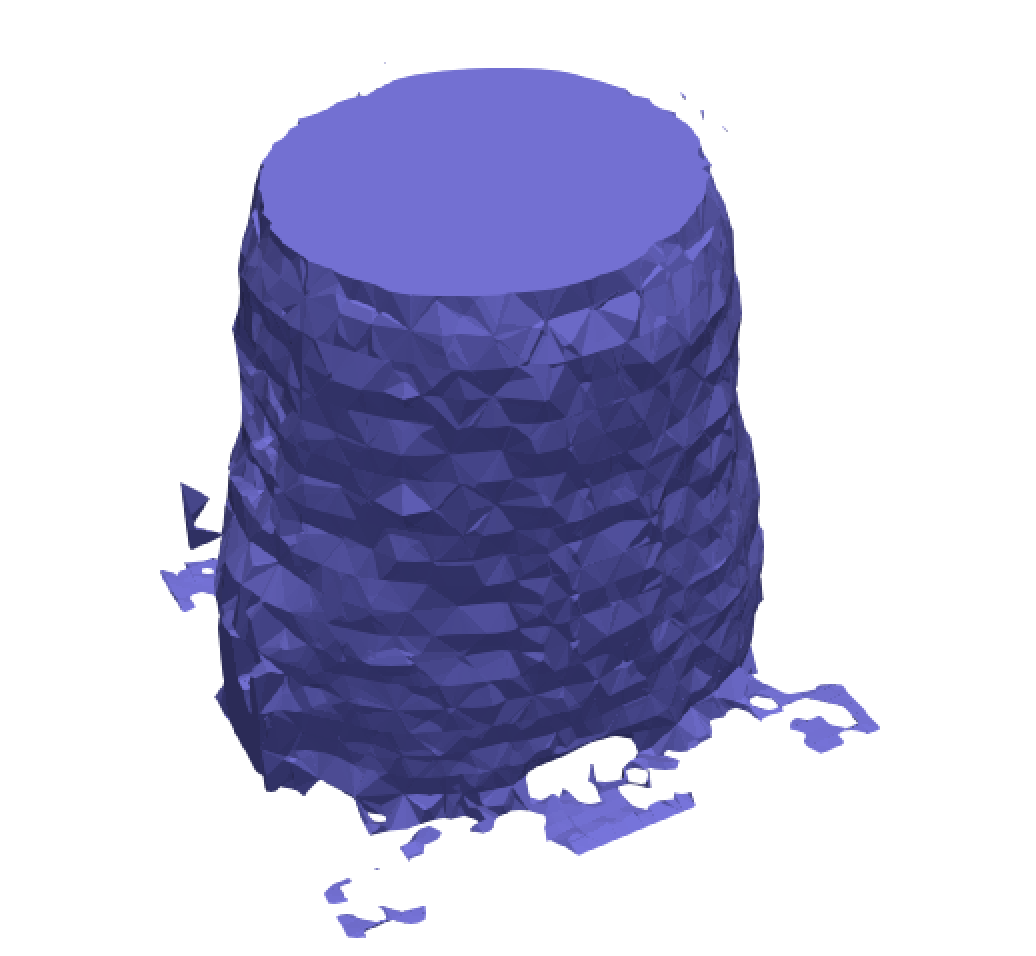
\includegraphics[width=0.6\textwidth]{tour}
		\caption{Optimisation de la compliance avec contrainte g\'eom\'etrique sur les couches}
	\end{minipage}
	\begin{minipage}{0.45\textwidth}
			\centering
			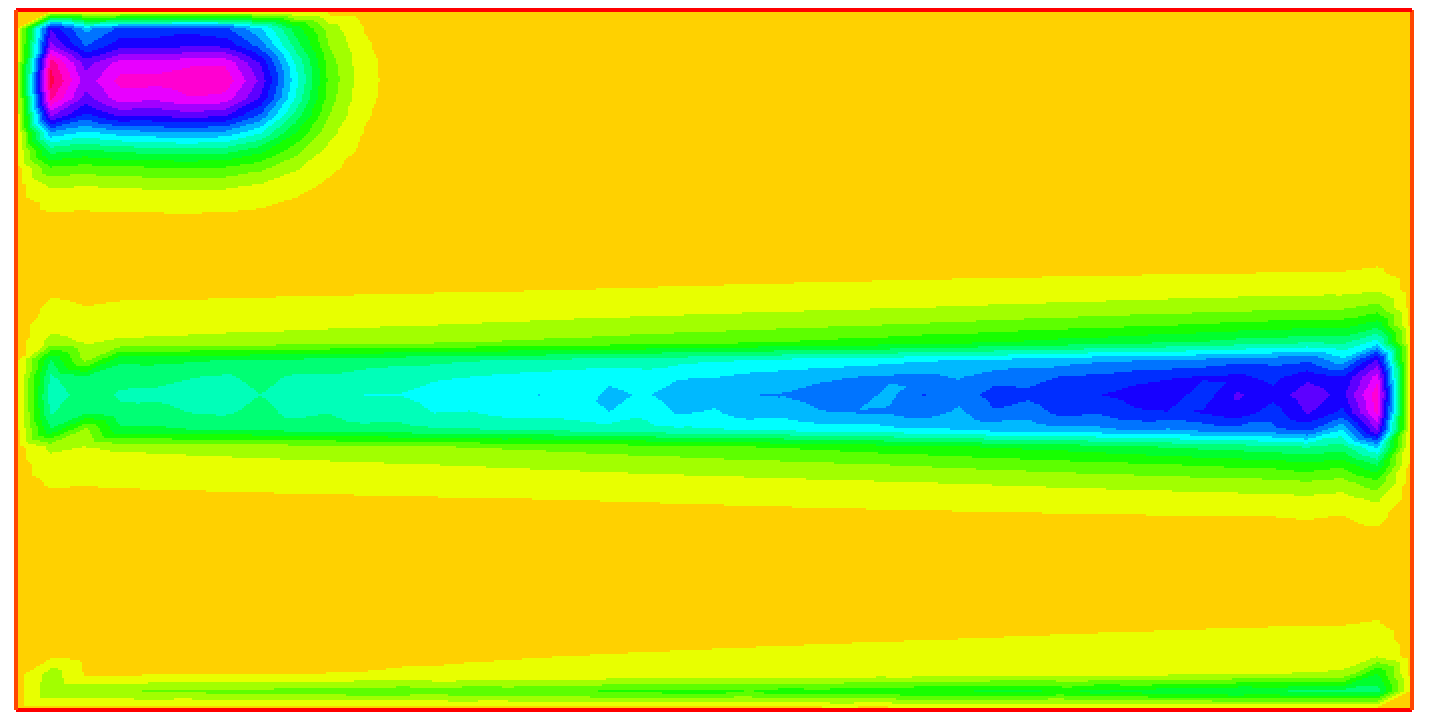
\includegraphics[width=0.9\textwidth]{temp}
			\caption{Mod\'elisation du passage d'un laser}
	\end{minipage}	
\end{figure}
%---------------------------------------------------------------
% REFERENCES BIBLIOGRAPHIQUES
%---------------------------------------------------------------
% NE PAS MODIFIER LES 2 LIGNES SUIVANTES
\bibliographystyle{plain}
\begin{thebibliography}{99}

\bibitem{ref1} {\sc G. Allaire, F. Jouve, A.-M. Toader,}, {\sl Structural optimization using sensitivity analysis and a level-set method}, J. Comp. Phys., Vol 194/1, pp.363-393, 2004.

\bibitem{ref2} {\sc M.Megahed, HW.Mindt, N.N’Dri, H.Duan, O.Desmaison}, {\sl Metal additive-manufacturing process and residual stress modeling}, Integrating Materials and Manufacturing Innovation, 5(1):4, décembre 2016.

% NE PAS MODIFIER LA LIGNE SUIVANTE
\end{thebibliography}
%
%---------------------------------------------------------------
% NOM & ADRESSE COMPLETE & EMAIL DU OU DES AUTEURS
% RETIRER LES SIGNES % SI NECESSAIRE ET PLACER DANS L'ORDRE SOUHAITE
% DANS LES LIGNES SUIVANTES NE MODIFIER QUE LES SIGNES COMMENTAIRES '%'
%---------------------------------------------------------------
\vfill
\auteurenbasdepage{\NomOrateur}{\AdresseLongueOrateur}{\EmailOrateur}
% Les noms, adresses, email de l'orateur et des co-auteurs sont a definir
% dans les macros \NomOrateur, \AdresseCourteOrateur etc. plus haut
%
\auteurenbasdepage{\NomAuteurI}{\AdresseLongueAuteurI}{\EmailAuteurI}
\auteurenbasdepage{\NomAuteurII}{\AdresseLongueAuteurII}{\EmailAuteurII}

%%%%%%%%%%%%%%%%%%%%%%%%%%%%%%%%%%%%%%%%%%%%%%%%%%%%%%%%%%%%%%%%%%%%%%%%%%%
\end{document}
